\documentclass{article}
\usepackage[utf8]{inputenc}


\title{Automatic Word Clustering Generation}
\author{
  Mello, Ney\\
  \texttt{neymello@gwu.edu}
  \and
  Sá, Lucas\\
  \texttt{lucastsa@gwu.edu}
  \and
  Silveira, José\\
  \texttt{silveiraneto@gwu.edu}
}
  \date{May 2013}

\usepackage{natbib}
\usepackage{graphicx}
\usepackage{float}

\begin{document}

\maketitle

\section{Introduction}
There is a theory which states that if ever anyone discovers exactly what
 the Universe is for and why it is here, 
it will instantly disappear and be replaced by something even more bizarre 
and inexplicable. \citep{kowalski2011information}

To develop this project, all algorithms were developed using pure Python. We found that Python was a very productive programming language for prototyping and experimenting the different approaches, which allowed us to move forward at a fast pace.

\section{The dataset}
% falar aqui sobre os dados de entrada. Histograma talvez. SIL %
The dataset consisted of a single file of 2315 lines representing 117 different documents. Each document representation inside the dataset was a excerpt of about 10 lines of pure text. The dataset was not case sensitive and all characters were in uppercase mode, both the text and titles. Each document has a title, used a key to reference to that particular documents. We found out that the titles were not unique though, making them not suitable to use as keys. This was circumvented using an additional counter append to each document title, making them unique and therefore approprieted to be used as keys.

\begin{figure}[h!]
    \centering
    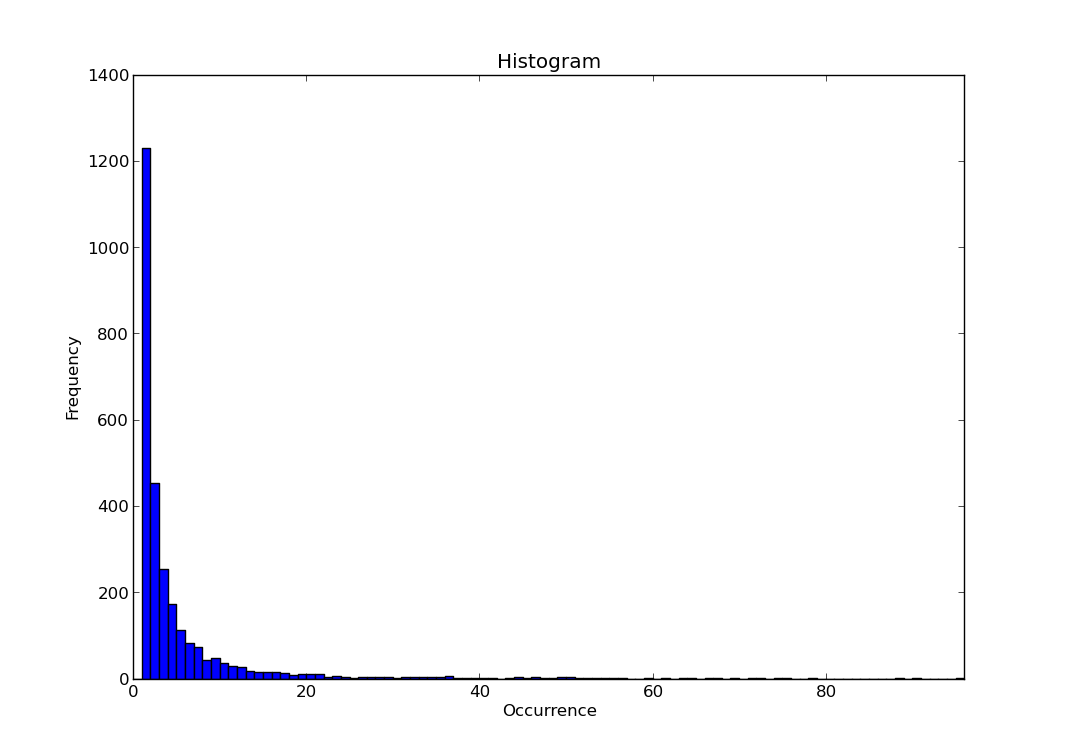
\includegraphics[scale=0.5]{histogram.png}
    \caption{Dataset frequency x ocurrence histogram graph}
    \label{fig:histogram}
\end{figure}
% da pra encher uma página aqui falando das palavras separadas sem nenhuma dica e como foi impossível contornar isso. SIL %

The analysis of the dataset revealed that a total 2806 unique words. These words are combined in 21996 words among the documents. In terms of frequency, there are 1229 words that appears only one time in the documents, and there are 1 word, the word \emph{THE}, that appear 1895 times. The complete histogram can be seen at Figure \ref{fig:histogram}. As we can see, there are a great number of ``rare'' words, i.e. words that rarely occur. There are 453 words that appear only 2 times, then 253 words that appear only 3 times, and so on. The logarithmical ratio betwen occurence and frequency is expected. The Figure \ref{fig:histogram} doesn't show in the horizontal axis values higher than 100 because they are too scattered and with low values. 

\begin{table}
    \centering
    \begin{tabular}{|c|c|}
    \hline
    word & frequency \\ \hline
    THE & 1895 \\ \hline
    OF   & 861 \\ \hline
    TO   & 713 \\ \hline
    A    & 603 \\ \hline
    IN   & 598 \\ \hline
    IS   & 427 \\ \hline
    AND  & 387 \\ \hline
    BE   & 337 \\ \hline
    THAT & 259 \\ \hline
    FOR  & 242 \\ \hline
    ARE  & 209 \\ \hline
    \end{tabular}
    \caption{Top 10 Words Frequency}
    \label{tab:top10}
\end{table}

As expected in a natural language dataset, the frequency of words are inversely proportional to their rank in number of occurrences, as stated by Zipf's law\cite{manning1999foundations}. Table \ref{tab:top10} shows the top 10 words by frequency. These words are frequent in any english document and therefore they don't aggregate semantically valuable indexing capability. This can be used as input for the list of words to ignore when processing the documents (the stop words list).

Additionally, words with a very low frequency do not present enough attributes for clustering purposes -- they lack co-occurence with other words in other documents, making it hard to detect correlation. As with any clustering algorithm, the analyzed underlying data requires a minimal number of observations in order to be considered statiscally relevant. Because of that, we limited our dataset to words that appears at least 7 times in the entire corpora.

With that limit, algorithms with very high order of complexity, such as the Clique algorithm, become computationally feasible due to the significant reduction in dimensionality (number of terms).

\section{Lexical analysis}

During the lexical analysis each dataset was treated as a sequence of characters and then converted into a sequence of tokens. In this project, each word that is not a title is considered a token. A set of algorithms and regular expression especially crafted for the peculiarities of our dataset were used to extract the tokens.

One particularity of our dataset is that in some documents the words were abruptly sliced at the end of the line without any special character of pattern to signalize these occurencies. Altough we tried some techniques as dictionary lookup, and pattern matching, we found them not feasible once we determined many cases of nondeterminism.

We also treated separately the body and title of the documents. Words in the titles were not considered as token because in our dataset they were not semantically relevant. We also had to add an extra identificator in the document titles so we could use them as keys, once the titles were not unique among the dataset.

The tokens were then indexed by document and later this data structure were used to create  the TF-IDF (\emph{Term Frequency–Inverse Document Frequency}) statistics.

\section{Similarity Measure}

The formula used to measure the between similarity between terms and terms is shown in Equation \ref{eq:sim}, where \emph{n} is the total number of terms. $Term_{x,y}$ is the frequency of the term \emph{y} in the document \emph{x}. This naïve similarity captures the idea that the more terms appear together in more documents, the more similar they are. Note that if there is no co-occurence of two terms in a document \emph{k}, then the product $(Term_{k,i})(Term_{k,j})$ is zero, i.e. only co-occurence is accounted.

\begin{equation} \label{eq:sim}
SIM(Term_{i}, Term_{j}) = \sum\limits_{k=1}^n (Term_{k,i})(Term_{k,j})
\end{equation}

Calculation the similarity measure for every pair of terms we produce the term-term matrix. Using this data structure we can easily access the precomputed values of similarity between any pair of terms. For our dataset, this is up to a 2806-by-2806 matrix if we don't remove any unique term from the analysis.

\subsection{Relationship Graph and Threshold}

Using a chosen threshold we generate a graph, where each vertice is a term and each edge between two vertices exist if there is a similarity greater than a chosen threshold in the term-term matrix. The graph will be more dense if there is more similarity between the terms and if we have lower threshold. On the other hand when we have less similarity and a higher threshold, we end up with a more sparse graph. There are two extreme scenarios: first, if the threshold is minimal then every two different vertices will be connected, in a single complete graph. If the threshold is maximal then no two vertices will be connected in the graph. 

\section{Clustering algorithms}



\subsection{Clique}
Description of Clique

\begin{figure}[H]
    \centering
    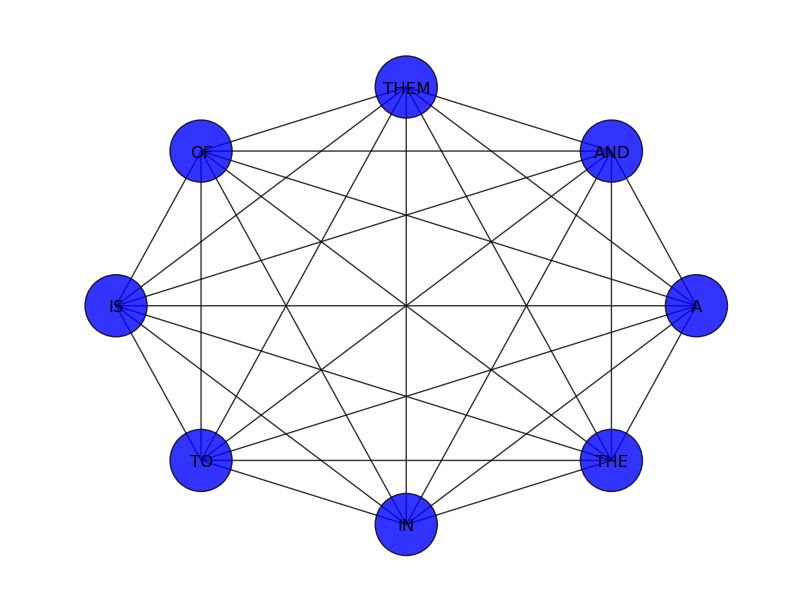
\includegraphics[scale=0.6]{clique_threshold150_size10_.png}
    \caption{An example of a Clique cluster of 10 words of the dataset, when the similarity threshold for term-relationship is 150.}
    \label{fig:example_clique}
\end{figure}

\subsection{Single-link}
Description of Single-link


\subsection{Star}
Description of Star

\begin{figure}[H]
    \centering
    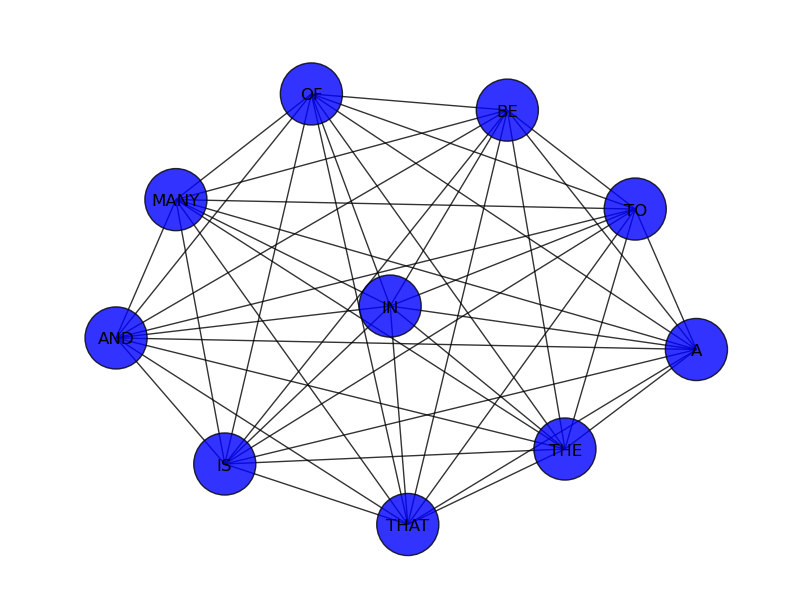
\includegraphics[scale=0.6]{star_threshold150_size10_.png}
    \caption{An example of a Star cluster of 10 words of the dataset, when the similarity threshold for term-relationship is 150.}
    \label{fig:example_star}
\end{figure}

\subsection{String}
Description of String

\begin{figure}[H]
    \centering
    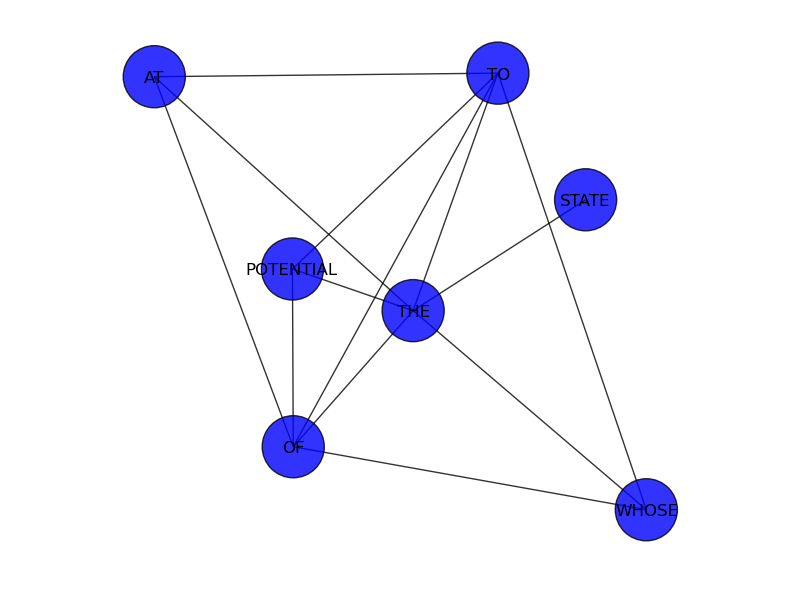
\includegraphics[scale=0.6]{string_threshold150_size7_.png}
    \caption{An example of a clique cluster of 7 words of the dataset, when the similarity threshold for term-relationship is 150.}
    \label{fig:example_string}
\end{figure}

\section{Results}

\begin{figure}[H]
    \centering
    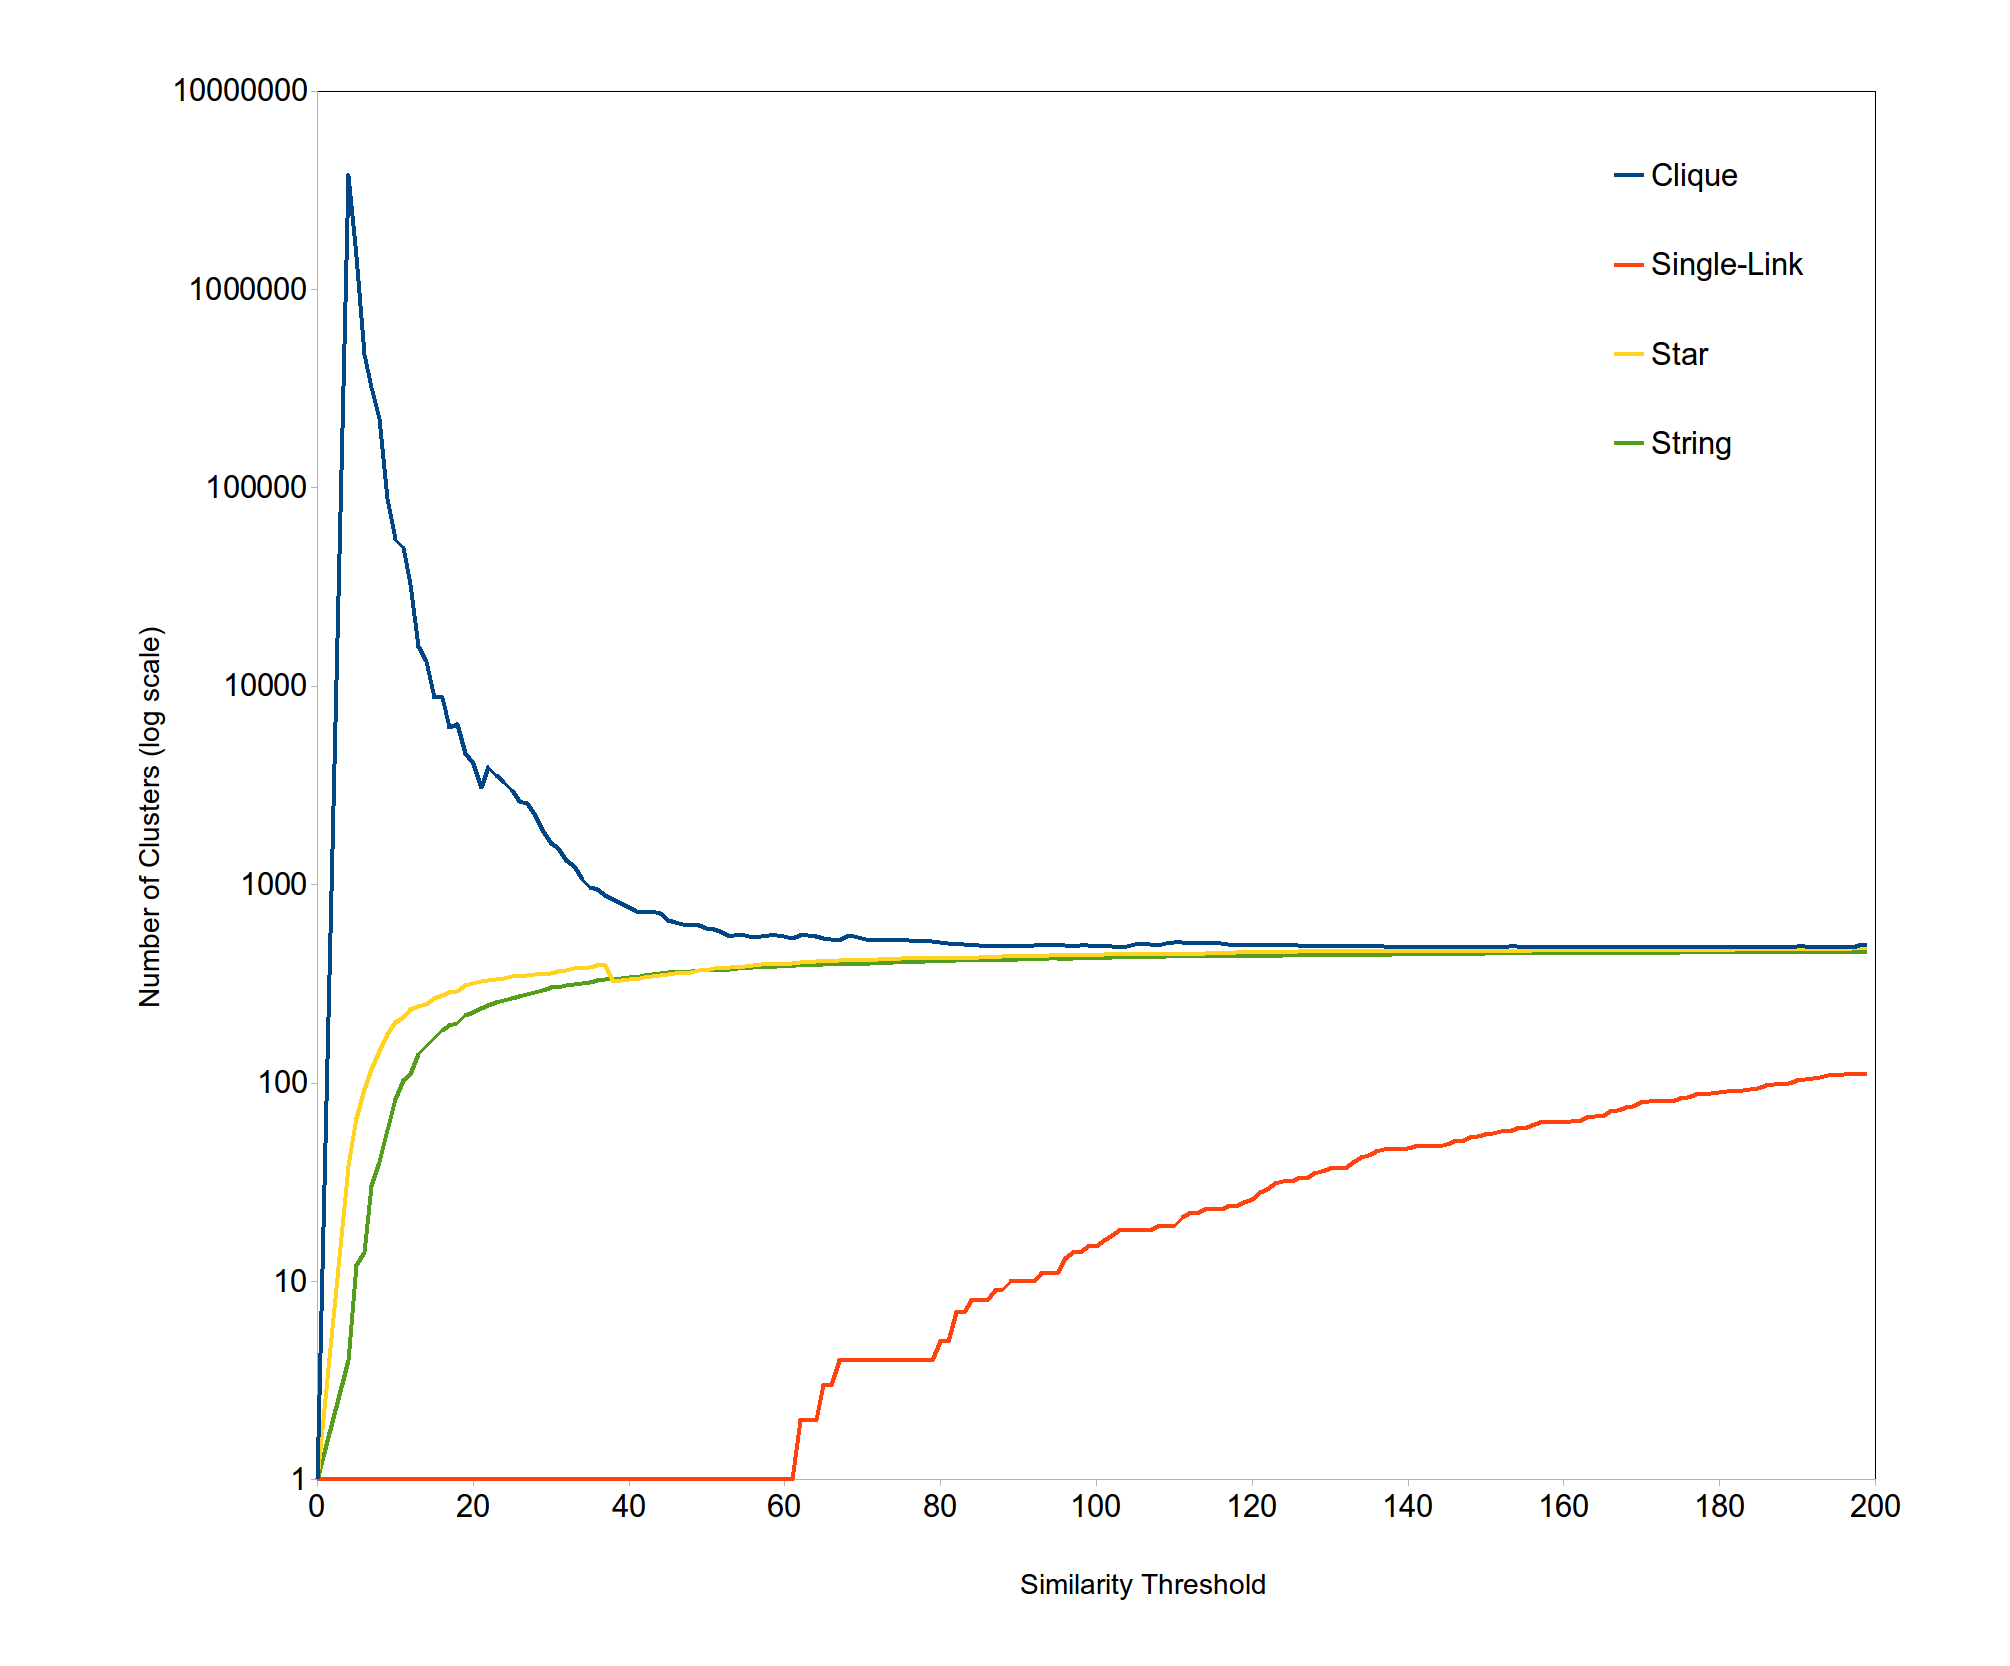
\includegraphics[scale=0.27]{similarity_threshold.png}
    \caption{Number of clusters generated by each algorithm with different similarities thresholds.}
    \label{fig:similarity_threshold}
\end{figure}

Brief discussion

\begin{figure}[H]
    \centering
    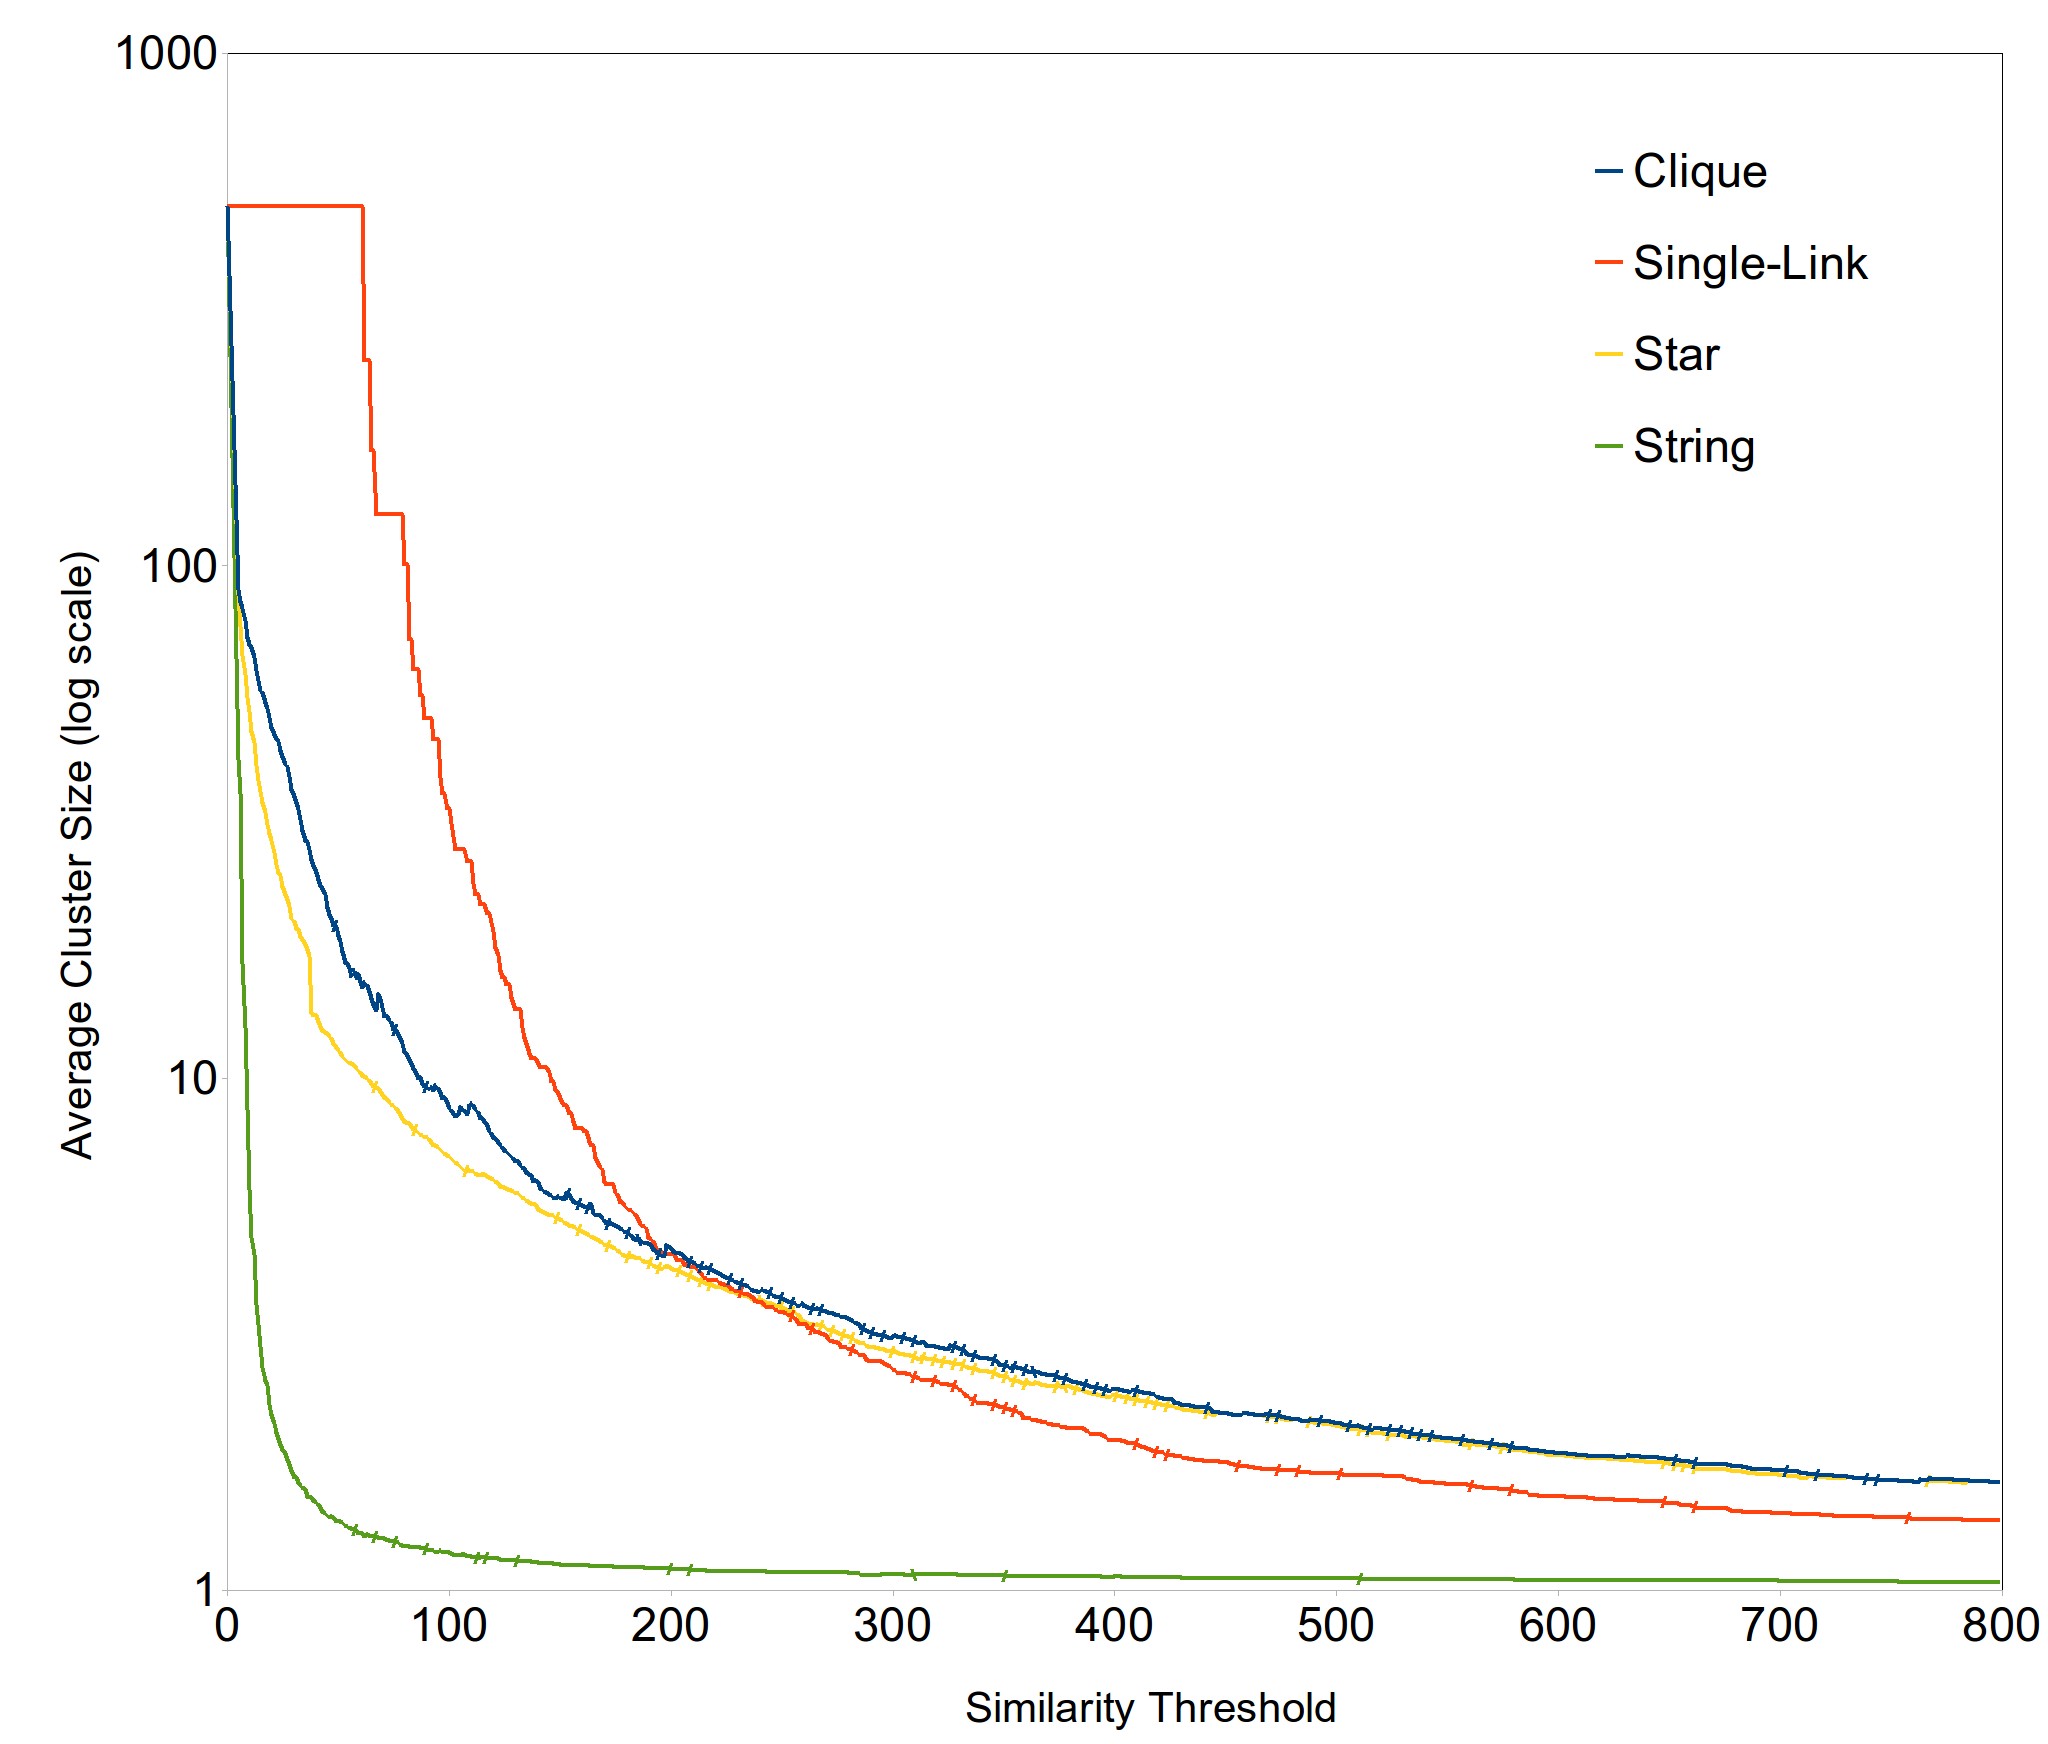
\includegraphics[scale=0.22]{size_by_similarity_threshold.png}
    \caption{Average size of clusters generated by each algorithm with different similarities thresholds.}
    \label{fig:size_by_similarity_threshold}
\end{figure}

Another interesting 
 
\section{Conclusion}
``I always thought something was fundamentally wrong with the universe'' 

\bibliographystyle{plain}
\bibliography{references}
\end{document}
